\section{Topics covered}
\begin{itemize}
\item Software pricing

\item Plan-driven development

\item Project scheduling

\item Agile planning

\item Estimation techniques
\end{itemize}
\section{Project planning}
\begin{itemize}
\item Project planning involves breaking down the work into parts and assign these to project team members, anticipate problems that might arise and prepare tentative solutions to those problems.

\item The project plan, which is created at the start of a project, is used to communicate how the work will be done to the project team and customers, and to help assess progress on the project.
\end{itemize}
\section{Planning stages}
\begin{itemize}

\item At the proposal stage, when you are bidding for a contract to develop or provide a software system.

\item During the project startup phase, when you have to plan who will work on the project, how the project will be broken down into increments, how resources will be allocated across your company, etc.

\item Periodically throughout the project, when you modify your plan in the light of experience gained and information from monitoring the progress of the work.

\end{itemize}
\section{Proposal planning}
\begin{itemize}

\item Planning may be necessary with only outline software requirements.

\item The aim of planning at this stage is to provide information that will be used in setting a price for the system to customers.
\end{itemize}
\section{Software pricing}
\begin{itemize}

\item Estimates are made to discover the cost, to the developer, of producing a software system.

  \item You take into account, hardware, software, travel, training and effort costs.

\item There is not a simple relationship between the development cost and the price charged to the customer.

\item Broader organisational, economic, political and business considerations influence the price charged.
\end{itemize}

\section{Plan-driven development}
\begin{itemize}

\item Plan-driven or plan-based development is an approach to software engineering where the development process is planned in detail.

  \item Plan-driven development is based on engineering project management techniques and is the ‘traditional’ way of managing large software development projects.

\item A project plan is created that records the work to be done, who will do it, the development schedule and the work products.

\item Managers use the plan to support project decision making and as a way of measuring progress.
\end{itemize}

\newpage
\section{Factors affecting software pricing}
\begin{table}[h!]
\centering
\begin{tabular}{ |p{3cm}|p{8cm}|  }
\hline
Factor & Description \\
\hline
\hline
Market opportunity & A development organization may quote a low price because it wishes to move into a new segment of the software market. Accepting a low profit on one project may give the organization the opportunity to make a greater profit later. The experience gained may also help it develop new products.\\
\hline
Cost estimate uncertainty & If an organization is unsure of its cost estimate, it may increase its price by a contingency over and above its normal profit.\\
\hline
Contractual terms & A customer may be willing to allow the developer to retain ownership of the source code and reuse it in other projects. The price charged may then be less than if the software source code is handed over to the customer.\\
\hline
Requirements volatility & If the requirements are likely to change, an organization may lower its price to win a contract. After the contract is awarded, high prices can be charged for changes to the requirements.\\
\hline
Financial health & Developers in financial difficulty may lower their price to gain a contract. It is better to make a smaller than normal profit or break even than to go out of business. Cash flow is more important than profit in difficult economic times.\\

\hline
\end{tabular}

\label{table:T6_1}
\end{table}

\section{Plan-driven development – pros and cons}
\begin{itemize}

\item The arguments in favor of a plan-driven approach are that early planning allows organizational issues (availability of staff, other projects, etc.) to be closely taken into account, and that potential problems and dependencies are discovered before the project starts, rather than once the project is underway.

\item The principal argument against plan-driven development is that many early decisions have to be revised because of changes to the environment in which the software is to be developed and used.
\end{itemize}
 \section{Project plans}
 \begin{itemize}

\item In a plan-driven development project, a project plan sets out the resources available to the project, the work breakdown and a schedule for carrying out the work.

\item Plan sections   \item Introduction   \item Project organization   \item Risk analysis
  \item Hardware and software resource requirements   \item Work breakdown
  \item Project schedule

  \item Monitoring and reporting mechanisms
\end{itemize}

% \newpage
\section{Project plan supplements}
\begin{table}[h!]
\centering
\begin{tabular}{ |p{3cm}|p{8cm}|  }
\hline
Plan & Description \\
\hline
\hline
Quality plan & Describes the quality procedures and standards that will be used in a project.\\
\hline
Validation plan & Describes the approach, resources, and schedule used for system validation.\\
\hline
Configuration management plan & Describes the configuration management procedures and structures to be used.\\
\hline
Maintenance plan & Predicts the maintenance requirements, costs, and effort.\\
\hline
Staff development plan & Describes how the skills and experience of the project team members will be developed.\\
\hline
\end{tabular}

\label{table:T6_2}
\end{table}

\section{The planning process}
\begin{itemize}

\item Project planning is an iterative process that starts when you create an initial project plan during the project startup phase.

\item Plan changes are inevitable.

  \item As more information about the system and the project team becomes available during the project, you should regularly revise the plan to reflect requirements, schedule and risk changes.
  \item Changing business goals also leads to changes in project plans. As business goals change, this could affect all projects, which may then have to be re-planned.
  \begin{figure}[h!]
      \centering
      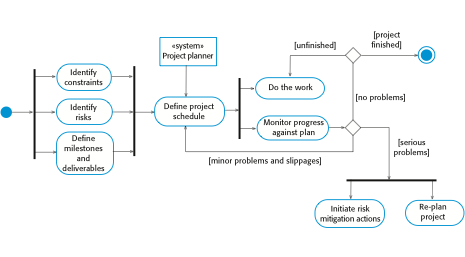
\includegraphics[width = 0.8\textwidth]{./figures/L6_1.png}
      \caption{}
      \label{fig:L6_1}
  \end{figure}

\end{itemize}
\section{Project scheduling}
\begin{itemize}

\item Project scheduling is the process of deciding how the work in a project will be organized as separate tasks, and when and how these tasks will be executed.

\item You estimate the calendar time needed to complete each task, the effort required and who will work on the tasks that have been identified.

\item You also have to estimate the resources needed to complete each task, such as the disk space required on a server, the time required on specialized hardware, such as a simulator, and what the travel budget will be.
\end{itemize}
\section{Project scheduling activities}
\begin{itemize}

\item Split project into tasks and estimate time and resources required to complete each task.

\item Organize tasks concurrently to make optimal use of workforce.

\item Minimize task dependencies to avoid delays caused by one task waiting for another to complete.

\item Dependent on project managers intuition and experience.
\end{itemize}
\section{Milestones and deliverables}
\begin{itemize}

\item Milestones are points in the schedule against which you can assess progress, for example, the handover of the system for testing.

\item Deliverables are work products that are delivered to the customer, e.g. a requirements document for the system.
\section{The project scheduling process}
\begin{figure}[h!]
    \centering
    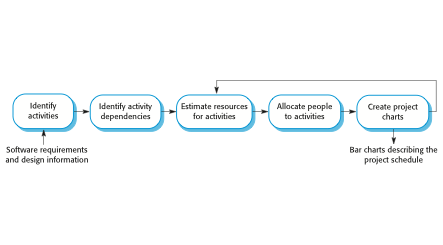
\includegraphics[width = 0.8\textwidth]{./figures/L6_2.png}
    \caption{}
    \label{fig:L6_2}
\end{figure}


\end{itemize}
\section{Scheduling problems}
\begin{itemize}

\item Estimating the difficulty of problems and hence the cost of developing a solution is hard.

\item Productivity is not proportional to the number of people working on a task.

\item Adding people to a late project makes it later because of communication overheads.

\item The unexpected always happens. Always allow contingency in planning.
\end{itemize}
\section{Schedule representation}
\begin{itemize}

\item Graphical notations are normally used to illustrate the project schedule.

\item These show the project breakdown into tasks. Tasks should not be too small. They should take about a week or two.

\item Bar charts are the most commonly used representation for project schedules. They show the schedule as activities or resources against time.
\end{itemize}
\section{Tasks, durations, and dependencies}
\begin{table}[h!]
\centering
\begin{tabular}{ |p{2cm}|p{2cm}|p{2cm}|p{3cm}|  }
\hline
Task & Effort (person-days) & Duration (days) &  Dependencies\\
\hline
\hline
T1 & 15 & 10 & \\
\hline
T2 & 8 & 15 & \\
\hline
T3 & 20 & 15 & T1 (M1)\\
\hline
T4 & 5 & 10 & \\
\hline
T5 & 5 & 10 & T2, T4 (M3)\\
\hline
T6 & 10 & 5 & T1, T2 (M4)\\
\hline
T7 & 25 & 20 & T1 (M1)\\
\hline
T8 & 75 & 25 & T4 (M2)\\
\hline
T9 & 10 & 15 & T3, T6 (M5)\\
\hline
T10 & 20 & 15 & T7, T8 (M6)\\
\hline
T11 & 10 & 10 & T9 (M7)\\
\hline
T12 & 20 & 10 & T10, T11 (M8)\\
\hline
\end{tabular}

\label{table:T6_2}
\end{table}



\newpage
\section{Activity bar chart}
\begin{figure}[h!]
    \centering
    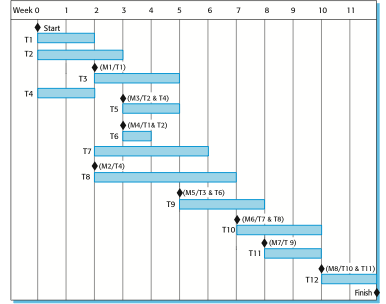
\includegraphics[width = 0.8\textwidth]{./figures/L6_3.png}
    \caption{}
    \label{fig:L6_3}
\end{figure}

\section{Staff allocation chart}
\begin{figure}[h!]
    \centering
    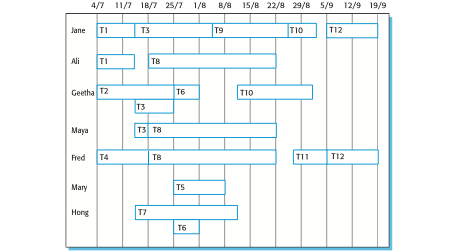
\includegraphics[width = 0.8\textwidth]{./figures/L6_4.png}
    \caption{}
    \label{fig:L6_4}
\end{figure}

\section{Agile planning}
\begin{itemize}

\item Agile methods of software development are iterative approaches where the software is developed and delivered to customers in increments.

\item Unlike plan-driven approaches, the functionality of these increments is not planned in advance but is decided during the development.

  \item The decision on what to include in an increment depends on progress and on the customer’s priorities.

\item The customer’s priorities and requirements change so it makes sense to have a flexible plan that can accommodate these changes.
\end{itemize}
\section{Agile planning stages}
\begin{itemize}

\item Release planning, which looks ahead for several months and decides on the features that should be included in a release of a system.

\item Iteration planning, which has a shorter term outlook, and focuses on planning the next increment of a system. This is typically 2-4 weeks of work for the team.
\end{itemize}

\section{Planning in XP}
\begin{figure}[h!]
    \centering
    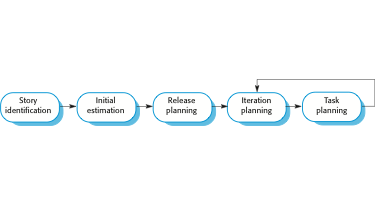
\includegraphics[width = 0.8\textwidth]{./figures/L6_5.png}
    \caption{}
    \label{fig:L6_5}
\end{figure}

\section{Story-based planning}
\begin{itemize}

\item The system specification in XP is based on user stories that reflect the features that should be included in the system.

\item The project team read and discuss the stories and rank them in order of the amount of time they think it will take to implement the story.

\item Release planning involves selecting and refining the stories that will reflect the features to be implemented in a release of a system and the order in which the stories should be implemented.

\item Stories to be implemented in each iteration are chosen, with the number of stories reflecting the time to deliver an iteration (usually 2 or 3 weeks).
\end{itemize}
\section{Key points}
\begin{itemize}

\item The price charged for a system does not just depend on its estimated development costs; it may be adjusted depending on the market and organizational priorities.

\item Plan-driven development is organized around a complete project plan that defines the project activities, the planned effort, the activity schedule and who is responsible for each activity.

\item Project scheduling involves the creation of graphical representations the project plan. Bar chartsshow the activity duration and staffing timelines, are the most commonly used schedule representations.

\item The XP planning game involves the whole team in project planning. The plan is developed incrementally and, if problems arise, is adjusted. Software functionality is reduced instead of delaying delivery of an increment.

\end{itemize}
\section{Estimation techniques}
\begin{itemize}

\item Organizations need to make software effort and cost estimates. There are two types of technique that can be used to do this:

  \item Experience-based techniques The estimate of future effort requirements is based on the manager’s experience of past projects and the application domain. Essentially, the manager makes an informed judgment of what the effort requirements are likely to be.
  \item Algorithmic cost modeling In this approach, a formulaic approach is used to compute the project effort based on estimates of product attributes, such as size, and process characteristics, such as experience of staff involved.
\end{itemize}
\section{Experience-based approaches}
\begin{itemize}

\item Experience-based techniques rely on judgments based on experience of past projects and the effort expended in these projects on software development activities.

\item Typically, you identify the deliverables to be produced in a project and the different software components or systems that are to be developed.

\item You document these in a spreadsheet, estimate them individually and compute the total effort required.

\item It usually helps to get a group of people involved in the effort estimation and to ask each member of the group to explain their estimate.
\end{itemize}
\section{Algorithmic cost modelling}
\begin{itemize}


\item Cost is estimated as a mathematical function of product, project and process attributes whose values are estimated by project managers:

  \item $Effort = A * Size^B * M$

  \item A is an organisation-dependent constant, B reflects the disproportionate effort for large projects and M is a multiplier reflecting product, process and people attributes.

\item The most commonly used product attribute for cost estimation is code size.

\item Most models are similar but they use different values for A, B and M.
\end{itemize}
\section{Estimation accuracy}
\begin{itemize}

\item The size of a software system can only be known accurately when it is finished.

\item Several factors influence the final size   \item Use of COTS and components;   \item Programming language;
  \item Distribution of system.

\item As the development process progresses then the size estimate becomes more accurate.

\item The estimates of the factors contributing to B and M are subjective and vary according to the judgment of the estimator.
\end{itemize}

\section{Estimate uncertainty}
\begin{figure}[h!]
    \centering
    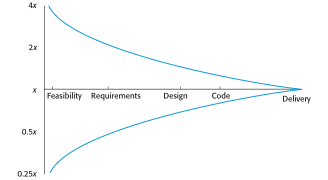
\includegraphics[width = 0.8\textwidth]{./figures/L6_6.png}
    \caption{}
    \label{fig:L6_6}
\end{figure}

\section{The COCOMO 2 model}
\begin{itemize}

\item An empirical model based on project experience.

\item Well-documented, ‘independent’ model which is not tied to a specific software vendor.

\item Long history from initial version published in 1981 (COCOMO-81) through various instantiations to COCOMO 2.

\item COCOMO 2 takes into account different approaches to software development, reuse, etc.
\end{itemize}
\section{COCOMO 2 models}
\begin{itemize}

\item COCOMO 2 incorporates a range of sub-models that produce increasingly detailed software estimates.

\item The sub-models in COCOMO 2 are:

  \item Application composition model. Used when software is composed from existing parts.
  \item Early design model. Used when requirements are available but design has not yet started.
  \item Reuse model. Used to compute the effort of integrating reusable components.
  \item Post-architecture model. Used once the system architecture has been designed and more information about the system is available.
\end{itemize}

\section{COCOMO estimation models}
\begin{figure}[h!]
    \centering
    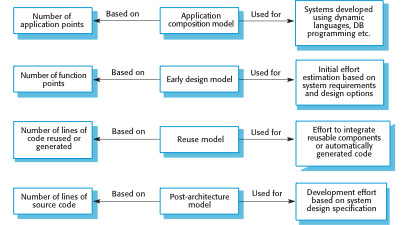
\includegraphics[width = 0.8\textwidth]{./figures/L6_7.png}
    \caption{}
    \label{fig:L6_7}
\end{figure}

\section{Application composition model}
\begin{itemize}
\item Supports prototyping projects and projects where there is extensive reuse.

\item Based on standard estimates of developer productivity in application (object) points/month.

\item Takes CASE tool use into account.

\item Formula is

  \item $ PM = \frac{( NAP * (1 - \% \frac{reuse}{100} ) )}{PROD}$

  \item PM is the effort in person-months, NAP is the number of application points and PROD is the productivity.
\end{itemize}

\newpage
\section{Application-point productivity}
\begin{table}[h!]
\centering
\begin{tabular}{ |p{2cm}|p{1cm}|p{1cm}|p{1cm}|p{1cm}|p{1cm}|  }
\hline
Developer’s experience and capability &  Very low & Low & Nominal & High & Very High\\
\hline
\hline
ICASE maturity and capability & Very low & Low & Nominal & High & Very high\\
\hline
PROD (NAP/month) & 4 & 7 & 13 & 25 & 50\\
\hline
\end{tabular}

\label{table:T6_3}
\end{table}

\section{Early design model}
\begin{itemize}

\item Estimates can be made after the requirements have been agreed.

\item Based on a standard formula for algorithmic models
\item $PM = A * SizeB * M$ where
  \item $M = PERS * RCPX * RUSE * PDIF * PREX * FCIL * SCED;$
  \item $A = 2.94$ in initial calibration, Size in KLOC, B varies from 1.1 to 1.24 depending on novelty of the project, development flexibility, risk management approaches and the process maturity.
\end{itemize}
 \section{Multipliers}
 \begin{itemize}

\item Multipliers reflect the capability of the developers, the non-functional requirements, the familiarity with the development platform, etc.

  \item RCPX - product reliability and complexity;   \item RUSE - the reuse required;
  \item PDIF - platform difficulty;   \item PREX - personnel experience;   \item PERS - personnel capability;   \item SCED - required schedule;   \item FCIL - the team support facilities.
\end{itemize}
\section{The reuse model}
\begin{itemize}

\item Takes into account black-box code that is reused without change and code that has to be adapted to integrate it with new code.

\item There are two versions:

  \item Black-box reuse where code is not modified. An effort estimate (PM) is computed.
  \item White-box reuse where code is modified. A size estimate equivalent to the number of lines of new source code is computed. This then adjusts the size estimate for new code.
\end{itemize}
\section{Reuse model estimates 1}
\begin{itemize}

\item For generated code:

  \item $PM = \frac{(ASLOC * \frac{AT}{100})}{ATPROD}$

  \item ASLOC is the number of lines of generated code   \item AT is the percentage of code automatically generated.
  \item ATPROD is the productivity of engineers in integrating this code.
\end{itemize}
\section{Reuse model estimates 2}
\begin{itemize}

\item When code has to be understood and integrated:
  \item $ESLOC = ASLOC * (1-\frac{AT}{100}) * AAM$
  \item ASLOC and AT as before.

  \item AAM is the adaptation adjustment multiplier computed from the costs of changing the reused code, the costs of understanding how to integrate the code and the costs of reuse decision making.
\end{itemize}
 \section{Post-architecture level}
 \begin{itemize}

\item Uses the same formula as the early design model but with 17 rather than 7 associated multipliers.

\item The code size is estimated as:

  \item Number of lines of new code to be developed;

  \item Estimate of equivalent number of lines of new code computed using the reuse model;
  \item An estimate of the number of lines of code that have to be modified according to requirements changes.
\end{itemize}
\section{The exponent term}
\begin{itemize}

\item This depends on 5 scale factors (see next slide). Their $\frac{sum}{100}$ is added to $1.01$

\item A company takes on a project in a new domain. The client has not defined the process to be used and has not allowed time for risk analysis. \end{itemize}
\section{The company has a CMM level 2 rating.}
\begin{itemize}

  \item Precedenteness - new project (4)
  \item Development flexibility - no client involvement - Very high (1)   \item Architecture/risk resolution - No risk analysis - V. Low .(5)   \item Team cohesion - new team - nominal (3)
  \item Process maturity - some control - nominal (3) \item Scale factor is therefore 1.17.
\end{itemize}

\section{Multipliers}
\begin{itemize}

\item Product attributes

  \item Concerned with required characteristics of the software product being developed.

\item Computer attributes

  \item Constraints imposed on the software by the hardware platform.

\item Personnel attributes

  \item Multipliers that take the experience and capabilities of the people working on the project into account.

\item Project attributes

  \item Concerned with the particular characteristics of the software development project.
\end{itemize}
\newpage
 \section{Scale factors used in the exponent computation in the post-architecture model}
 \begin{table}[h!]
 \centering
 \begin{tabular}{ |p{3cm}|p{8cm}|  }
 \hline
 Scale factor & Explanation\\
 \hline
 \hline
 Precedentedness & Reflects the previous experience of the organization with this type of project. Very low means no previous experience; extra-high means that the organization is completely familiar with this application domain.\\
 \hline
 Development flexibility & Reflects the degree of flexibility in the development process. Very low means a prescribed process is used; extra-high means that the client sets only general goals.\\
 \hline
 Architecture/risk resolution & Reflects the extent of risk analysis carried out. Very low means little analysis; extra-high means a complete and thorough risk analysis.\\
 \hline
 Team cohesion & Reflects how well the development team knows each other and work together. Very low means very difficult interactions; extra-high means an integrated and effective team with no communication problems.\\
 \hline
 Process maturity & Reflects the process maturity of the organization. The computation of this value depends on the CMM Maturity Questionnaire, but an estimate can be achieved by subtracting the CMM process maturity level from 5.\\
 \hline
 \end{tabular}

 \label{table:T6_4}
 \end{table}

\newpage
\section{The effect of cost drivers on effort estimates}
\begin{table}[h!]
\centering
\begin{tabular}{ |p{3cm}|p{8cm}|  }
\hline
Exponent value & 1.17\\
\hline
\hline
System size (including factors for reuse and requirements volatility) & 128,000 DSI\\
\hline
Initial COCOMO estimate without cost drivers & 730 person-months\\
\hline
Reliability & Very high, multiplier = 1.39\\
\hline
Complexity & Very high, multiplier = 1.3\\
\hline
Memory constraint & High, multiplier = 1.21\\
\hline
Tool use & Low, multiplier = 1.12\\
\hline
Schedule & Accelerated, multiplier = 1.29\\
\hline
Adjusted COCOMO estimate & 2,306 person-months\\
\hline
\hline
Reliability & Very low, multiplier = 0.75\\
\hline
Complexity & Very low, multiplier = 0.75\\
\hline
Memory constraint & None, multiplier = 1\\
\hline
Tool use & Very high, multiplier = 0.72\\
\hline
Schedule & Normal, multiplier = 1\\
\hline
Adjusted COCOMO estimate & 295 person-months\\
\hline
\end{tabular}

\label{table:T6_4}
\end{table}

\section{Project duration and staffing}
\begin{itemize}

\item As well as effort estimation, managers must estimate the calendar time required to complete a project and when staff will be required.
\item Calendar time can be estimated using a COCOMO 2 formula
\item TDEV = 3 * (PM)(0.33+0.2*(B-1.01))
\item PM is the effort computation and B is the exponent computed as discussed above (B is 1 for the early prototyping model). This computation predicts the nominal schedule for the project.
\item The time required is independent of the number of people working on the project.

\end{itemize}

\section{Staffing requirements}
\begin{itemize}

\item Staff required can’t be computed by diving the development time by the required schedule.

\item The number of people working on a project varies depending on the phase of the project.

\item The more people who work on the project, the more total effort is usually required.

\item A very rapid build-up of people often correlates with schedule slippage.
\end{itemize}
\section{Key points}
\begin{itemize}

\item Estimation techniques for software may be experience-based, where managers judge the effort required, or algorithmic, where the effort required is computed from other estimated project parameters.

\item The COCOMO II costing model is an algorithmic cost model that uses project, product, hardware and personnel attributes as well as product size and complexity attributes to derive a cost estimate.
\end{itemize}
